
%(BEGIN_QUESTION)
% Copyright 2007, Tony R. Kuphaldt, released under the Creative Commons Attribution License (v 1.0)
% This means you may do almost anything with this work of mine, so long as you give me proper credit

Examine the following oxygen trim control system (with cross-limiting for safety), and then answer the questions that follow:

$$\includegraphics[width=15.5cm]{i01829x01.eps}$$

\begin{itemize}
\item{} What is the purpose of the two select relays?
\item{} Do the flow controllers need to be direct-acting or reverse-acting, assuming signal-to-open control valves?
\item{} Does the oxygen controller (AIC) need to be direct-acting or reverse-acting?
\item{} What will happen if the oxygen analyzer fails in a state with the output saturated at 100\% (maximum oxygen)?
\end{itemize}

\vskip 20pt \vbox{\hrule \hbox{\strut \vrule{} {\bf Suggestions for Socratic discussion} \vrule} \hrule}

\begin{itemize}
\item{} It is usually a bad idea to include a multiplier relay inside a control loop, such as shown in this oxygen trim control system.  Placing a multiplier function inside of a control loop changes the gain of that loop, which can lead to instability.  However, it is a reasonably safe thing to do here, inside the air flow control loop.  Explain why.
\end{itemize}

\underbar{file i01829}
%(END_QUESTION)





%(BEGIN_ANSWER)

The two ``select'' relays ensure the air/fuel ratio will always err on the side of too lean (instead of too rich) during quick changes in firing rate demand.  

\vskip 10pt

Both flow controllers need to be {\it reverse} acting.

\vskip 10pt

The oxygen controller needs to be {\it direct} acting.

%(END_ANSWER)





%(BEGIN_NOTES)

The reason that the oxygen controller (AIC) needs to be direct acting may be proven through a thought experiment: imagine if the oxygen content of the flue gas is too high -- what action should the controller take.  Obviously, the controller should act to reduce the air:fuel ratio, either by decreasing air flow, increasing fuel flow, or both.  An increasing signal to the multiplier relay will do this, because it will make the air flow controller think there is too much air, thus cutting back on the air damper.  So, if we wish the controller to output a greater signal given a greater PV, we need that controller to be direct-acting.

\vskip 10pt

If the oxygen transmitter fails high, the system will act as though the mixture is too lean, and will work to make it richer.

\vskip 10pt

Challenge answer: oxygen trim control systems are usually not given much sway over air/fuel ratio, so the gain of the air flow control loop will not change enough to really make a difference in stability.

%INDEX% Control, strategies: oxygen trim control
%INDEX% Process: combustion furnace

%(END_NOTES)


